\section{Tor § Onion v2}
\begin{frame}{Tor}
    \begin{wrapfigure}{1}{0.2\textwidth}
        \centering
        
\includegraphics[width=0.2\textwidth]{TorLogo}
    \end{wrapfigure}

    La rete Tor è la più famosa implementazione di Onion, grazie all'apporto delle seguenti migliorie:
    \begin{itemize}
        \item Circuiti telescopici
        \item Proxy di applicazione tramite SOCKS
        \item Controllo di congestione
        \item Directory server
        \item Politiche di uscita variabili
        \item Controllo d'integrità end-to-end
    \end{itemize}
\end{frame}

\subsection{Obiettivi}
\begin{frame}{Obiettivi}
    L'obiettivo principale della rete TOR è quello di garantire l'anonimato dell'utente finale, e scoraggiare eventuali attaccanti, sono stati quindi definiti i seguenti obiettivi:
    \begin{itemize}
        \item Usabilità, la rete deve essere utilizzabile da chiunque, questo è un'aspetto fffondamentale per garantire l'anonimato.
        \item Semplicità, la rete deve essere semplice da utilizzare, in modo da non scoraggiare gli utenti meno esperti.
    \end{itemize}
\end{frame}

\subsection{Network Design}
\begin{frame}{Network Design}
    \begin{wrapfigure}{1}{0.2\textwidth}
        \centering
        \includesvg[width=0.3\textwidth]{overlayNetwork}
    \end{wrapfigure}

    La rete Tor è una rete che esiste al di sopra delle reti esistenti, per questo viene chiamata overlay network. I pacchetti TOR sono chiamati celle, sono di dimensione fissa 512 bytes, ci sono due tipi di celle:
    \begin{itemize}
        \item \textbf{Control}, gestisce la connessione
        \item \textbf{Relay}, trasporta stream dati
    \end{itemize}
    L'header oltre all'ID del circuito possiede un campo comando che indica come gestire il payload
    \begin{itemize}
        \item Padding, mantiene viva la connessione
        \item Create, crea un circuito
        \item Destroy, distrugge un circuito
    \end{itemize}
\end{frame}

\begin{frame}{Generazione del circuito}
    L'onion Proxy per generare un circuito segue un processo di negoziazione incrementale
    \begin{enumerate}
        \item Invia una richiesta relay al primo nodo
        \item Avviene la condivisione della chiave simmetrica tramite l'handshake di Diffie-Hellman con la conseguente generazione dell'ID del circuito
        \item Viene inviata una richiesta Relay \textbf{Extend} indicando l'indirizzo del secondo nodo
        \item Iterativamente vengono inviate altre richieste Relay Extend finché il circuito non è completo
    \end{enumerate}
    Da qui l'Onion Proxy inizia a gestire le richieste di applicazione
\end{frame}

\begin{frame}{Controllo di congestione}
    Non potendo in una rete Onion cambiare un router quando non è più in grado di gestire il carico, è stato necessario implementare un controllo di congestione che blocca i circuiti o gli stream dati quando questi inviano troppi dati usando due finestre:
    \begin{itemize}
        \item Packaging window, tiene traccia del numero di celle che un OR può inviare all'OP,     viene decrementata ad ogni cella verso l'OP ricevuta e incrementata ad ogni relay sendme ricevuto (dall'OP), quando raggiunge 0 smette di leggere e inoltrare celle
        \item Delivery window, tiene traccia del numero di celle che un OR può inviare fuori dalla rete
    \end{itemize}
    L'unica differenza tra i due controlli è la dimensione delle finestre e se si riferisce al circuito o allo stream.
\end{frame}

\begin{frame}{Tor Relay}
    La rete TOR si basa su un insieme di nodi gestiti da volontari chiamati TOR Relay, possono essere di tre tipi:
    \begin{itemize}
        \item \textbf{Non-exit Relay}, i nodi interni della rete che a loro volta si dividono in:
        \begin{itemize}
            \item \textbf{Guard Relay}, il primo nodo del circuito
            \item \textbf{Middle Relay}, i nodi intermedi del circuito
        \end{itemize}
        \item \textbf{Exit Relay}, i nodi di uscita della rete Tor, instradano il traffico nella rete comune. Essendo gli unici IP visibili all'esterno sono i più esposti a rischi legali.
        \item \textbf{Bridge Relay}, nodi non pubblici che non possono quindi essere bloccati
    \end{itemize}
    Tutte le informazioni sui Relay esistenti sono visitabili al seguente indirizzo: \url{https://metrics.torproject.org/rs.html}

\end{frame}

\begin{frame}{Directory Servers} 
    I Directory Server sono un sottogruppo di onion router che tracciano i cambiamenti nella \textbf{topologia di rete} e agiscono da \textbf{DNS server} per i servizi onion.
    Mantengono infatti i \textbf{descriptor}, pacchetti generati dai servizi onion criptati con la propria chiave privata, che contengono gli introduction points e la chiave pubblica.\\
    
    Il sistema di generazione di indirizzi onion fornisce un \textbf{meccanismo di sicurezza} per evitare che un malintenzionato possa alterare i descriptor e reindirizzare gli utenti ai propri introduction points, infatti se cosi fosse la chiave pubblica nascosta nell'indirizzo onion non sarebbe in grado di decifrare il descriptor.
\end{frame}

\subsection{Dimostrazione Wireshark}

\begin{frame}{Dimostrazione Wireshark}
    In Wireshark possiamo vedere il Client Hello, l'inizio della connessione con il server, in cui il client invia alcune informazioni tra cui la versione di TLS, la lista dei Cipher Suite supportati e la chiave pubblica.
    Possiamo poi vedere il Server Hello, ovvero la risposta del server con le relative informazioni di criptografia. \\
    Successivamente Tor usa le informazioni ottenute per stabilire una connessione TLS tra client e server, impedendoci di vedere il traffico dati.
\end{frame}

\begin{frame} 
    \begin{figure}
        \centering
        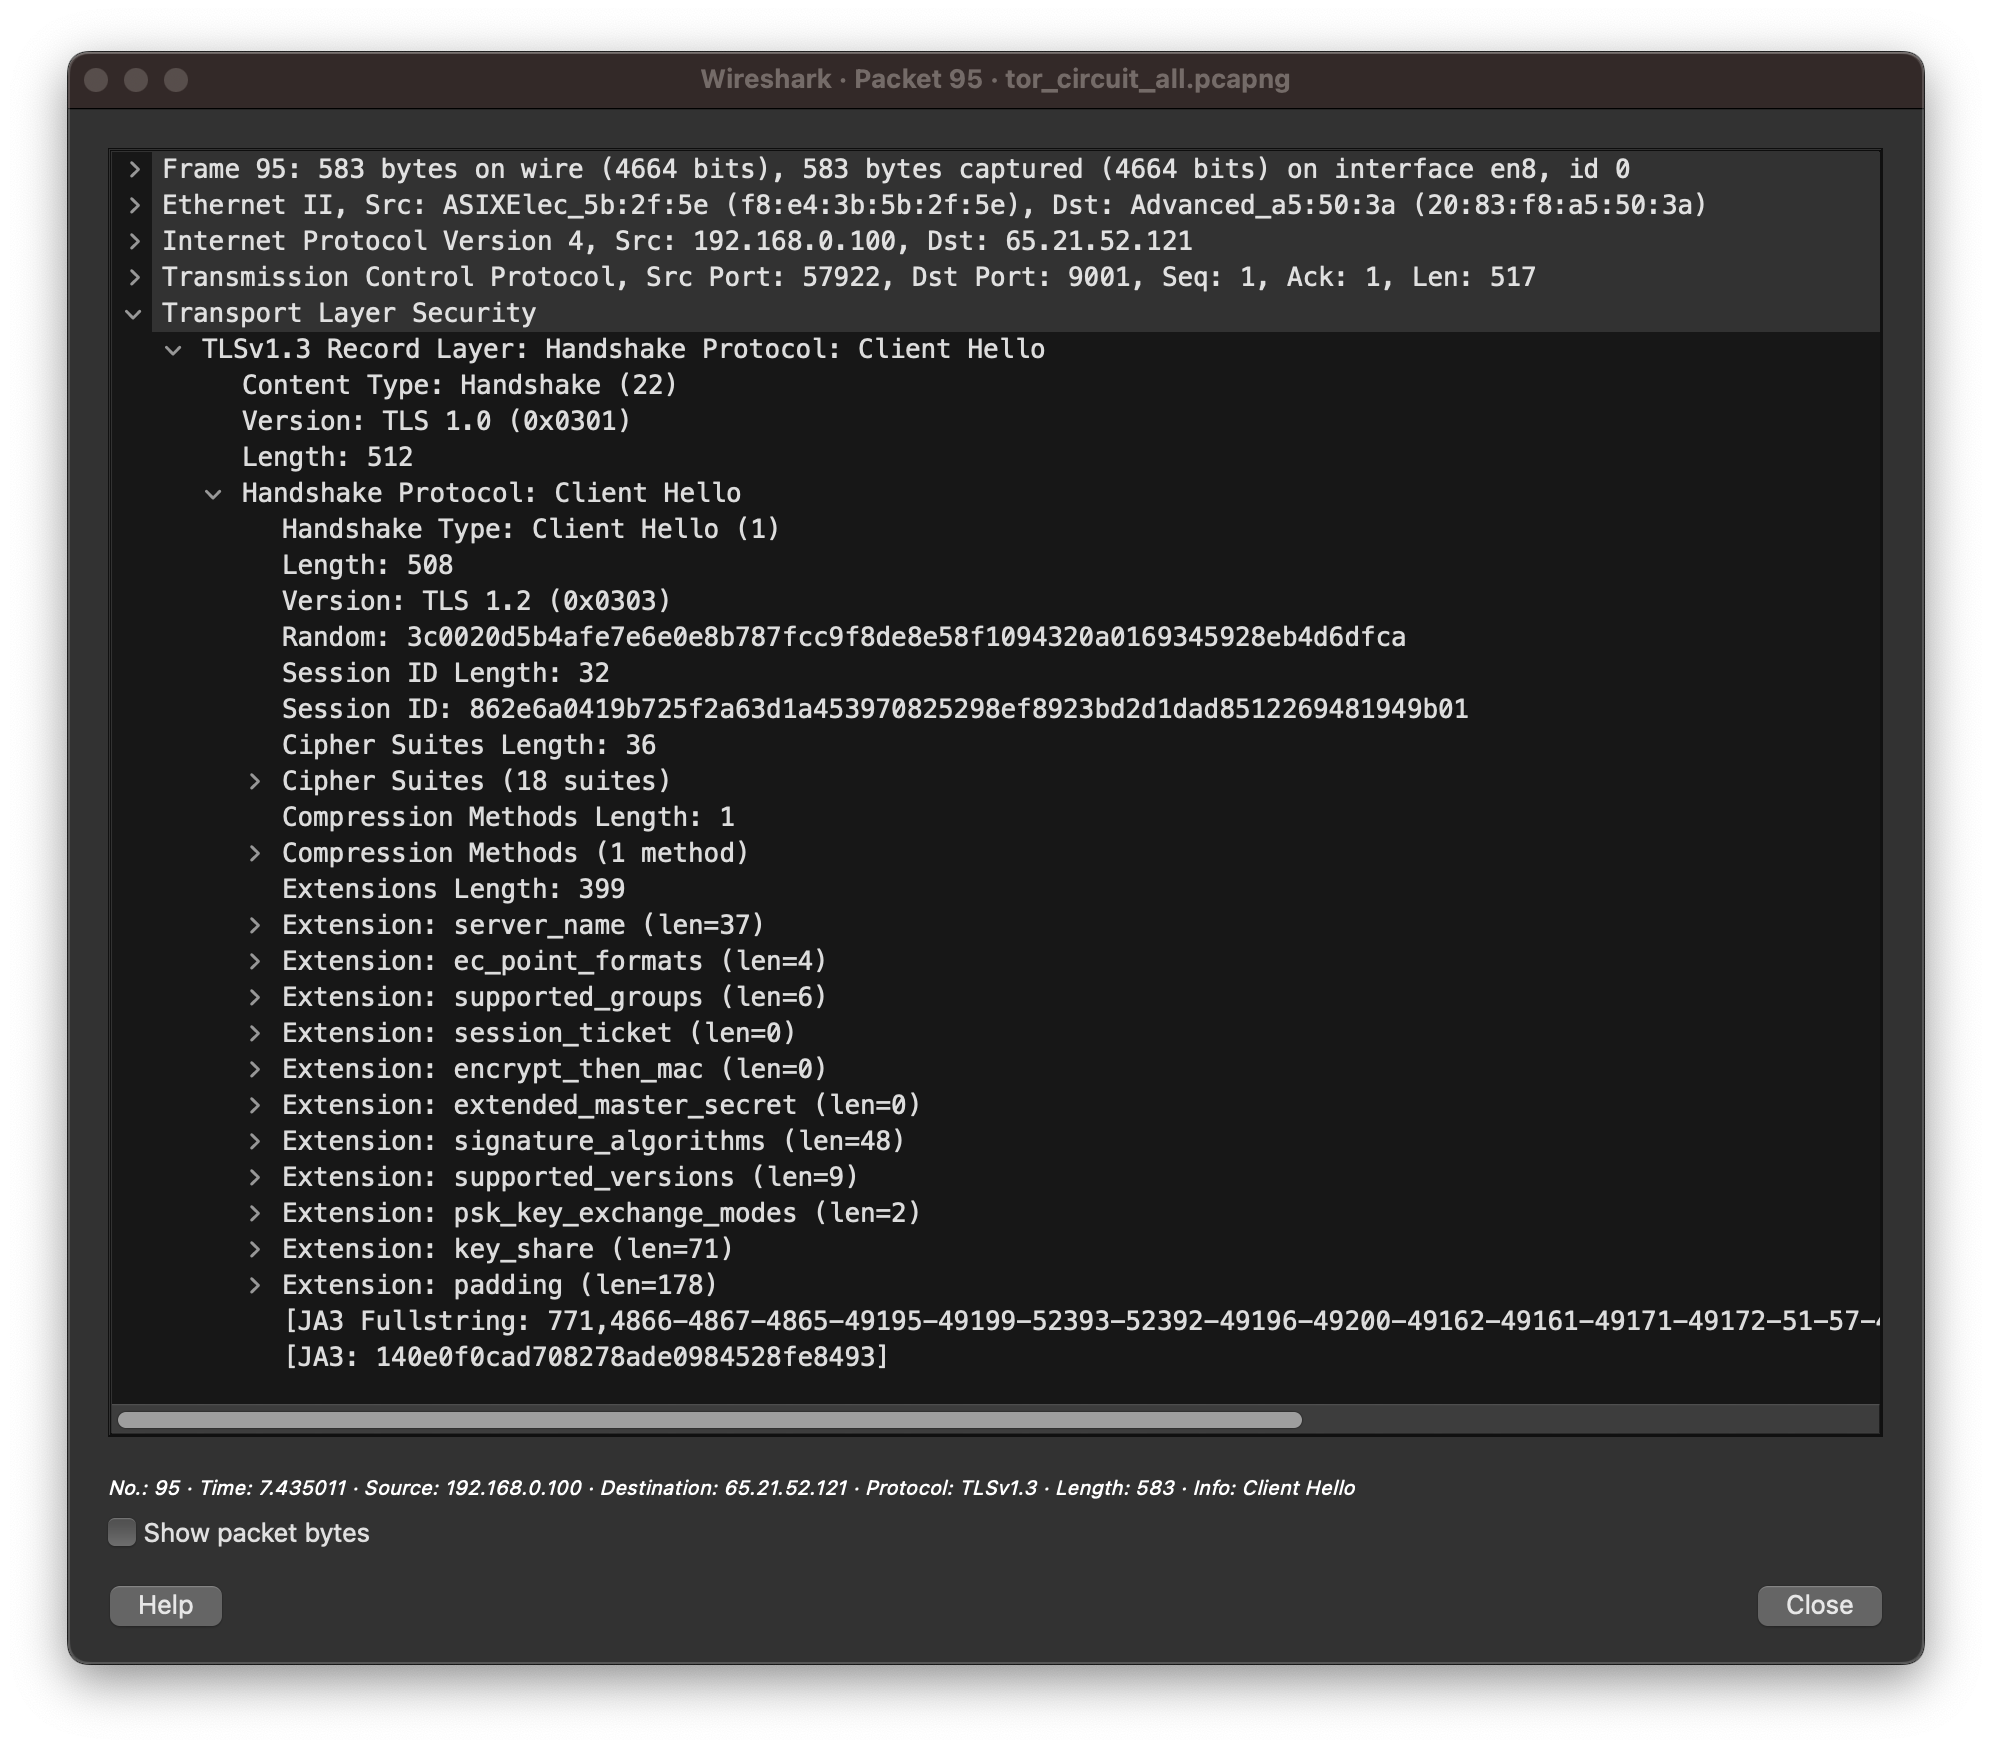
\includegraphics[width=0.9\textwidth]{Wireshark/Client_Hello}
    \end{figure}
\end{frame}

\begin{frame} 
    \begin{figure}
        \centering
        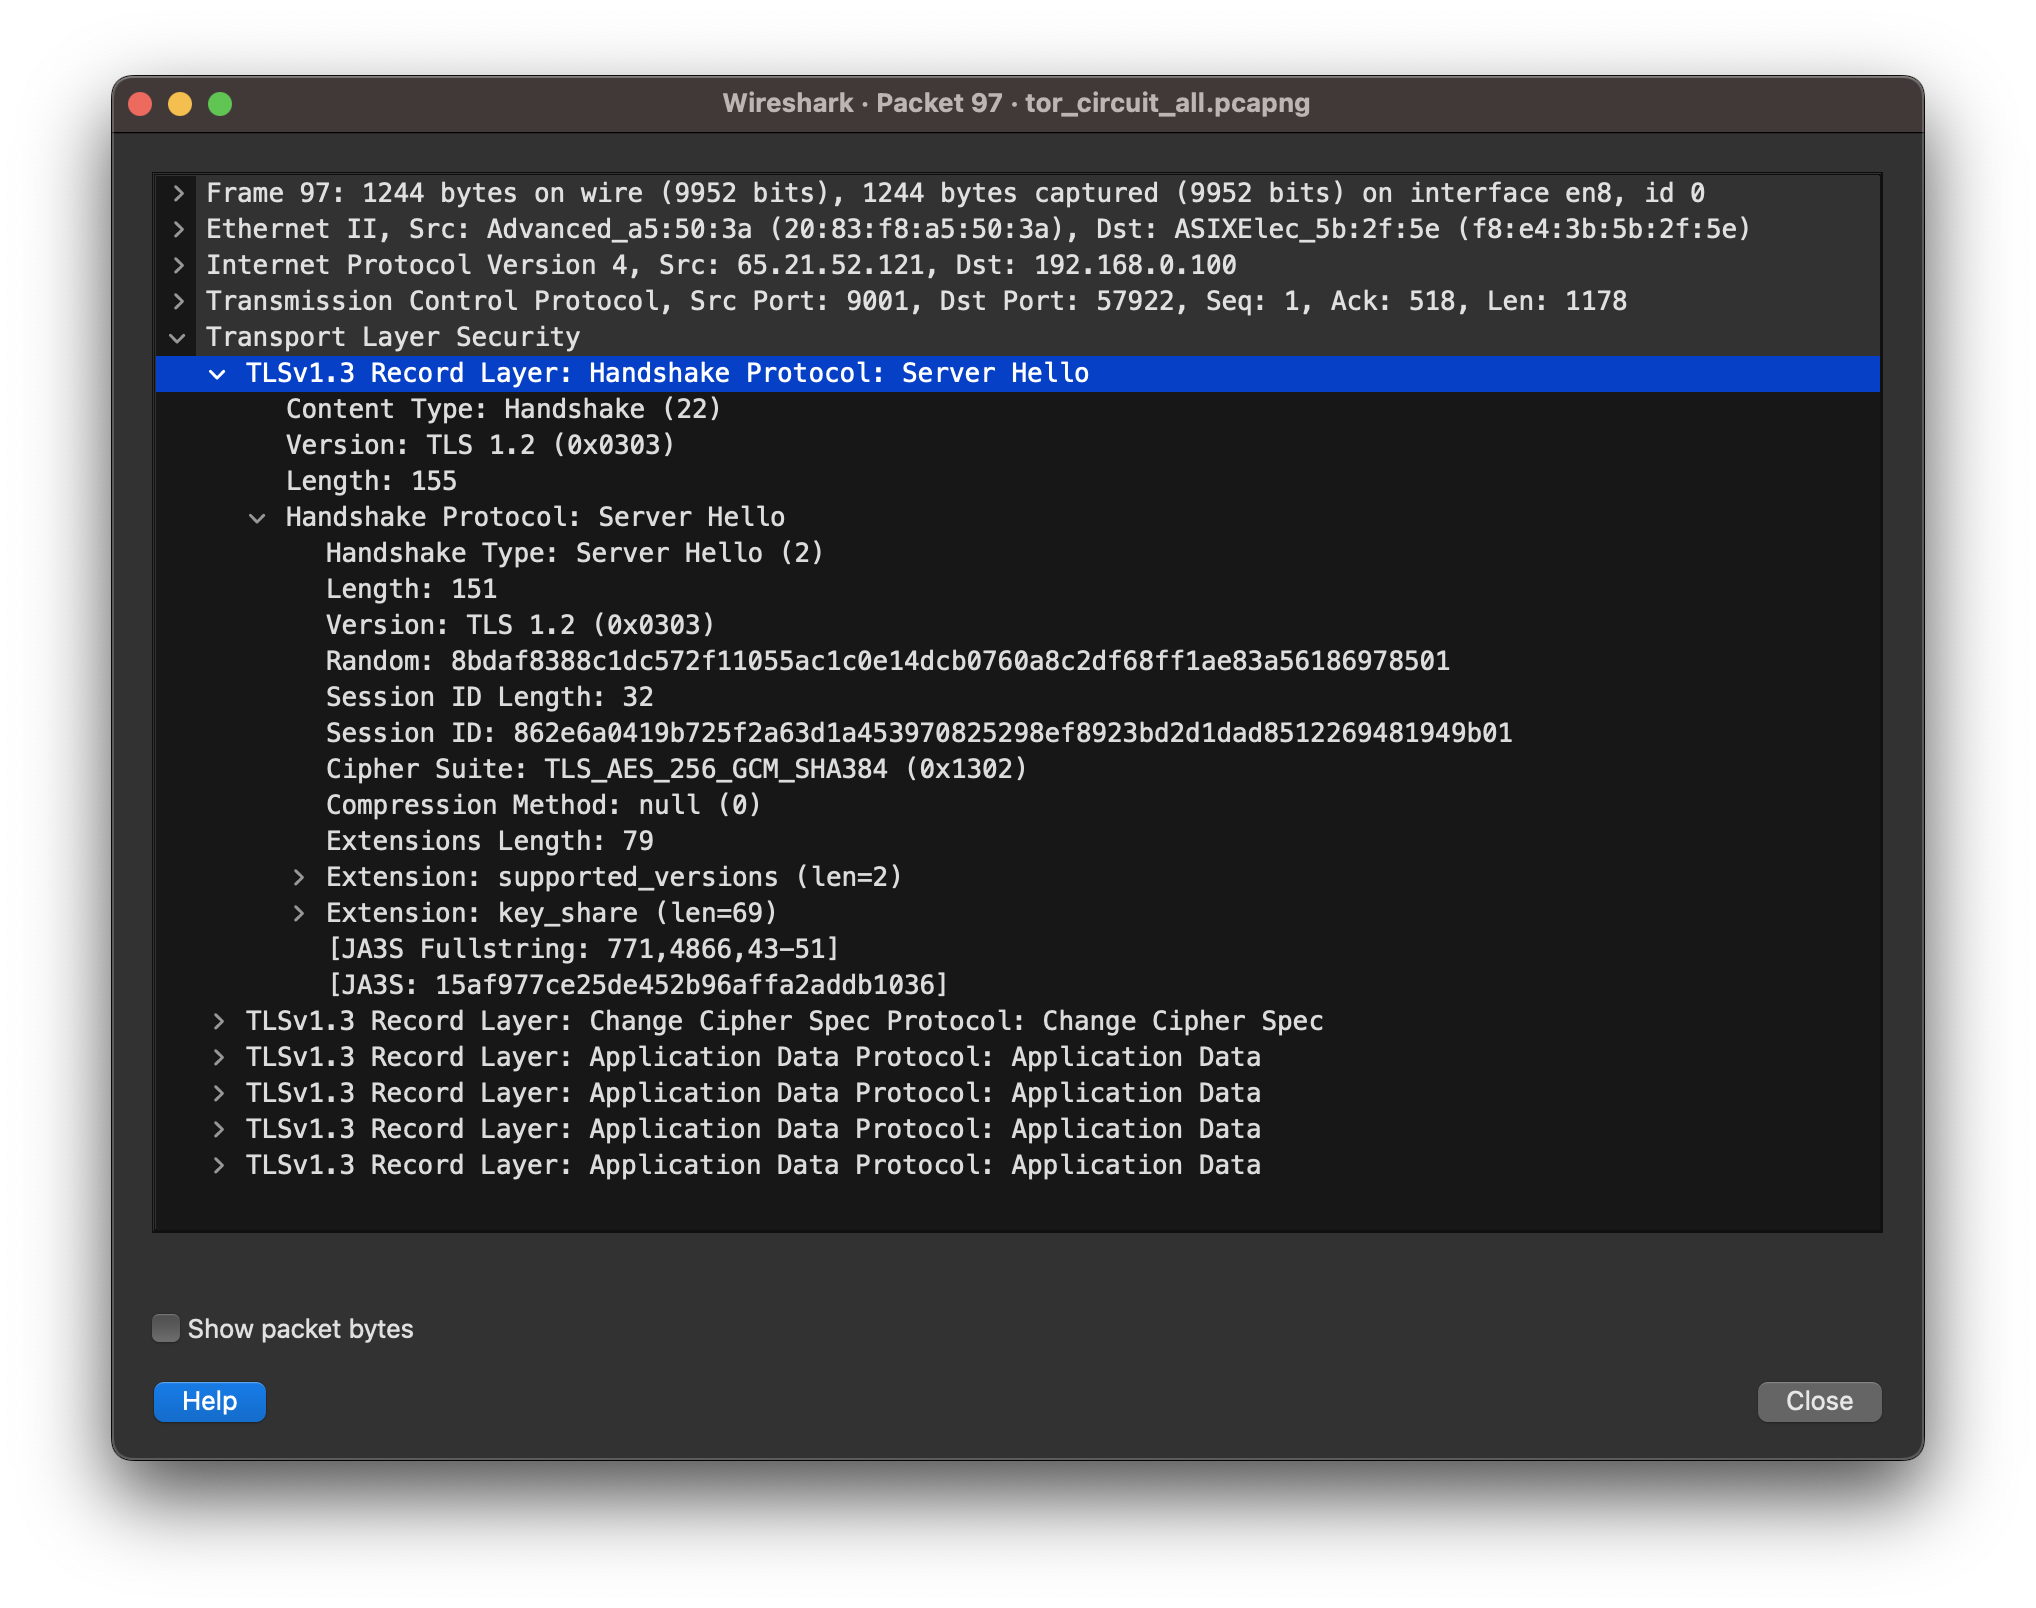
\includegraphics[width=0.7\textwidth]{Wireshark/Server_Hello}
    \end{figure}
\end{frame}
